\documentclass[12pt]{article}
\usepackage[tbtags]{amsmath}
\usepackage{graphicx}
\usepackage{enumerate}
\usepackage{natbib}
\usepackage{url}
\usepackage{authblk}

%\pdfminorversion=4
% NOTE: To produce blinded version, replace "0" with "1" below.
\newcommand{\blind}{0}

% DON'T change margins - should be 1 inch all around.
\addtolength{\oddsidemargin}{-.5in}%
\addtolength{\evensidemargin}{-.5in}%
\addtolength{\textwidth}{1in}%
\addtolength{\textheight}{-.3in}%
\addtolength{\topmargin}{-.8in}%

\DeclareMathOperator{\argmax}{arg\,max}
\DeclareMathOperator{\argmin}{arg\,min}

\begin{document}

%\bibliographystyle{natbib}

\def\spacingset#1{\renewcommand{\baselinestretch}%
{#1}\small\normalsize} \spacingset{1}


%%%%%%%%%%%%%%%%%%%%%%%%%%%%%%%%%%%%%%%%%%%%%%%%%%%%%%%%%%%%%%%%%%%%%%%%%%%%%%

\if0\blind
{
  \title{\bf Personalized Schedules for Burdensome Surveillance Tests}

\author[1]{Anirudh Tomer\footnote{Corresponding author: a.tomer@erasmusmc.nl\\The authors gratefully acknowledge Nederlandse Organisatie voor Wetenschappelijk Onderzoek VIDI grant nr. 016.146.301, and Erasmus University Medical Center funding.}}
\author[2]{Daan Nieboer}
\author[3]{Monique J. Roobol}
\author[2,4]{Ewout W. Steyerberg}
\author[1]{Dimitris Rizopoulos}

\affil[1]{Department of Biostatistics, Erasmus University Medical Center, the Netherlands}
\affil[2]{Department of Public Health, Erasmus University Medical Center, the Netherlands}
\affil[3]{Department of Urology, Erasmus University Medical Center, the Netherlands}
\affil[4]{Department of Biomedical Data Sciences, Leiden University Medical Center, the Netherlands}


  %\author{Anirudh Tomer\thanks{
    %The authors gratefully acknowledge \textit{please remember to list all relevant funding sources in the unblinded version}}\hspace{.2cm}\\
  %  Department of Biostatistics, Erasmus University Medical Center, the Netherlands\\
   % Daan Nieboer \\
   % Department of Public Health, Erasmus University Medical Center, the Netherlands\\
    %Monique J. Roobol \\
   % Department of Urology, Erasmus University Medical Center, the Netherlands \\
   % Ewout W. Steyerberg}

  \maketitle
} \fi

\if1\blind
{
  \bigskip
  \bigskip
  \bigskip
  \begin{center}
    {\LARGE\bf Personalized Schedules for Burdensome Surveillance Tests}
\end{center}
  \medskip
} \fi

\bigskip
% !TEX root =  ../main_manuscript.tex 
\begin{abstract}
\texttt{Objective}: To develop a model and methodology for predicting the risk of Gleason \emph{upgrading} in prostate cancer active surveillance (AS) patients, and using the predicted risks to create risk-based \emph{personalized} biopsy schedules as an alternative to one-size-fits-all schedules (e.g., annually). Furthermore, to assist patients and doctors in making shared decisions of biopsy schedules, by providing them quantitative estimates of the \emph{burden} and \emph{benefit} of opting for personalized versus any other schedule in AS. Last, to externally validate our model and implement it along with personalized schedules in a ready to use web-application.\\

\texttt{Materials and Methods}: We used longitudinal prostate-specific antigen (PSA) measurements, timing and results of previous biopsies, and age at baseline from the world's largest AS study, Prostate Cancer Research International Active Surveillance or PRIAS (7813 patients, 1134 experienced upgrading). We fitted a Bayesian joint model for time-to-event and longitudinal data to the PRIAS dataset. We then externally validated our model in the largest six AS cohorts of the Movember Foundation's Global Action Plan (GAP3) database (${>20,000}$ patients, 27 centers worldwide), covering nearly 73\% of all GAP3 patients. We used the predicted upgrading-risks from the validated models to schedule biopsies whenever a patient's risk of upgrading was above a certain threshold. To assist patients in choice of this threshold to compare the resulting schedule with currently practiced schedules, we provided them the timing and the total number of biopsies (burden) planned, and the predicted time delay in detecting upgrading (shorter is better) for each schedule.\\

\texttt{Results}: The cause-specific cumulative upgrading-risk at year five of follow-up was 35\% in PRIAS, and at most 50\% in GAP3 cohorts. In the PRIAS based model, PSA velocity was a stronger predictor of upgrading (Hazard~Ratio:~2.47, 95\%CI:~1.93--2.99) than PSA value (Hazard~Ratio:~0.99, 95\%CI:~0.89--1.11). Our model had a moderate area under the receiver operating characteristic curve (0.6--0.7) in validation cohorts. The prediction error was moderate (0.1--0.2) in GAP3 cohorts where the impact of PSA value and velocity on upgrading-risk was similar to PRIAS, but large (0.2--0.3) otherwise. Our model required recalibration of baseline upgrading-risk in validation cohorts. We used predicted upgrading-risk from the validated model to create personalized biopsy schedules for real AS patients and implemented them in a web-application (\url{http://tiny.cc/biopsy}).\\

\texttt{Conclusions}: We successfully developed and validated a model for predicting upgrading-risk, and providing risk-based personalized biopsy decisions, in prostate cancer AS. Personalized prostate biopsies are a novel alternative to fixed one-size-fits-all schedules that may help to reduce unnecessary prostate biopsies while maintaining cancer control. The model and schedules made available via a web-application enable shared decision making of biopsy schedules by comparing fixed and personalized schedules on total biopsies and expected time delay in detecting upgrading.
\end{abstract}

\noindent%
{\it Keywords:} Chronic NCDs, Invasive diagnostic tests, Joint models, Personalized schedules, Prostate biopsy, Surveillance
\vfill

\newpage
\spacingset{1.5} % DON'T change the spacing!

% !TEX root =  ../main_manuscript.tex 
\section{Introduction}
\label{sec:introduction}
Chronic non-communicable diseases (e.g., cancer, renal, cardiovascular diseases, etc.) are the primary cause of human deaths worldwide~\citep{alwan2010monitoring}. After diagnosis, in many such patients, surveillance tests are performed periodically to detect disease \textit{progression}, a non-terminal event. Often the most accurate or gold standard surveillance tests are also invasive. For example, to diagnose progression, biopsies are conducted repeatedly in prostate cancer~\citep{bokhorst2015compliance}, endoscopies in Barrett's esophagus~\citep{streitz1993endoscopic}, and colonoscopies in colorectal cancer~\citep{krist2007timing}. Repeat biopsies are also utilized to detect allograft deterioration in lung~\citep{mcwilliams2008surveillance} and kidney transplant~\citep{henderson2011surveillance} patients.

Usually, invasive tests are scheduled in a fixed manner, e.g., every six months. Test frequency varies between diseases~\citep{henderson2011surveillance,bokhorst2015compliance,krist2007timing} and cohorts. Although, due to the periodical nature of test schedules, progression is always detected with a time delay (Figure~\ref{fig:delay_explanation}). This time delay can be reduced by scheduling tests frequently. However, invasive tests are difficult to conduct, can lead to severe complications~\citep{loeb2013systematic,krist2007timing}, cause patient discomfort, and sometimes patients may not comply with frequent tests~\citep{bokhorst2015compliance}. In this regard, fixed test schedules ignore the differences in speed of progression between patients, and impose an equal medical burden on all. Hence, the frequency of invasive tests holds important implications for patients.

\begin{figure}
\centerline{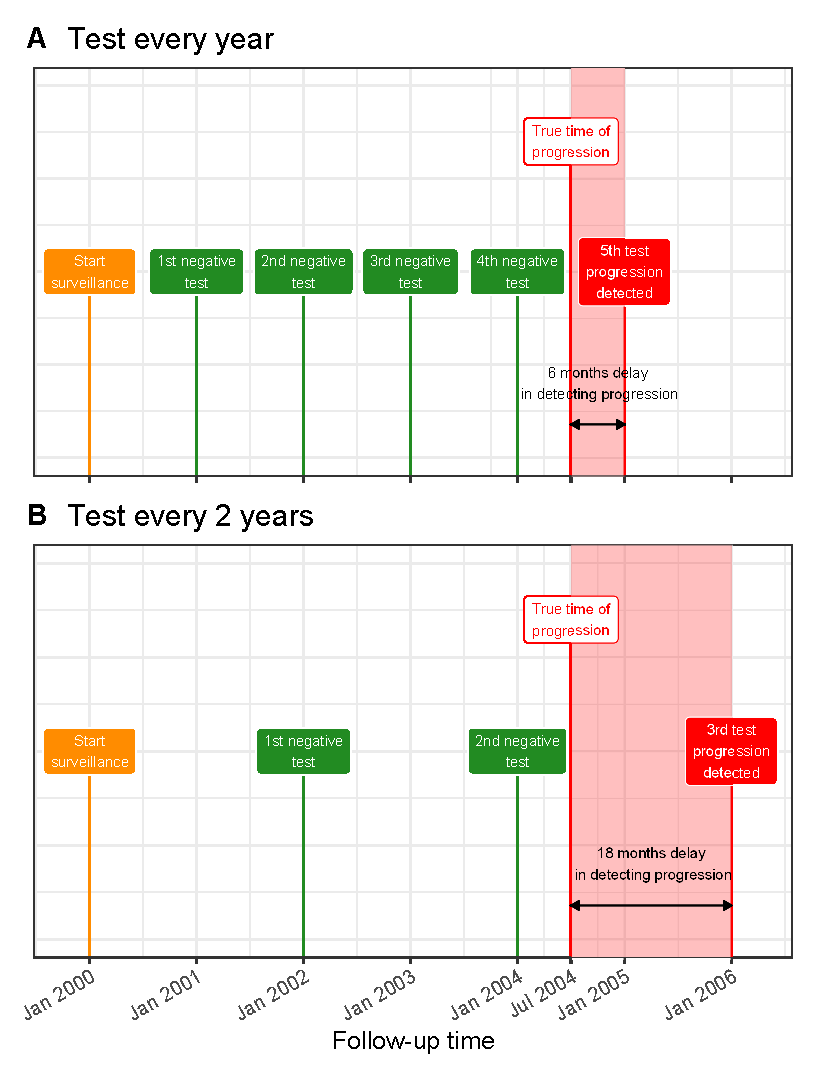
\includegraphics{images/delay_explanation.eps}}
\caption{\textbf{Trade-off between the number of invasive tests and time delay in detecting progression (non-terminal event of interest):} The true time of progression for this patient July 2004. More frequent invasive tests in \textbf{Panel~A} lead to a smaller time delay in detection of progression than less frequent invasive tests in \textbf{Panel~B}. Since invasive tests are conducted periodically, the time of progression is observed as an interval. For example, between Jan~2004--Jan~2005 in \textbf{Panel~A} and between Jan~2004--Jan~2006 in \textbf{Panel~B}.} 
\label{fig:delay_explanation}
\end{figure}

In this paper, we aim to balance the number of invasive tests (burden) and the time delay in detection of \textit{progression} (less is beneficial) better than fixed schedules. For this purpose, we intend to create personalized test schedules that exploit patient-specific clinical data accumulated during follow-up. This data includes baseline characteristics of patients; results from previous invasive tests; and longitudinal biomarker, physical examination, and medical imaging measurements, etc. Previous approaches for personalized schedules may be divided into three categories. First, heuristic methods such as decision making flowcharts, e.g.,~\citet{bokhorst2015compliance}. However, flowcharts discretize continuous clinical outcomes, often utilize only the latest data point, and ignore the measurement error in observed outcomes. Second, personalized test decisions employing partially observable Markov decision processes~\citep{alagoz2010operations, steimle2017markov}. Although, their application with continuous outcomes is limited by the curse of dimensionality. Third, personalized schedules obtained by optimizing a loss function of clinical parameters of interest~\citep{bebu2017optimal,rizopoulos2015personalized}, including our previous work on scheduling biopsies in prostate cancer~\citep{tomer2019personalized}. In this work, we will employ the third approach.

First, we develop a full specification of the joint distribution of patient-specific longitudinal clinical outcomes and time of \textit{progression}. We achieve this using joint models for time-to-event and longitudinal data~\citep{tsiatis2004joint,rizopoulos2012joint}. We use joint models because they are inherently personalized. Specifically, they exploit patient-specific random effects~\citep{laird1982random} to model longitudinal outcomes without discretizing them. We subsequently employ the fitted joint model for new patients, to estimate their patient-specific cumulative-risk over their current and future follow-up visits. These risk predictions utilize their clinical data accumulated until their latest follow-up. We then schedule invasive tests on all those future follow-up visits where a patient's conditional cumulative-risk of progression is above a certain threshold (e.g., 10\% risk). We also automate the choice of this threshold and the resulting schedule. More specifically, we optimize a function of the number of tests in a schedule and the expected time delay in the detection of progression. We estimate this delay in a patient-specific manner for both fixed and personalized schedules, thus facilitating shared-decision making of invasive test schedules.

This research is motivated by the problem of scheduling biopsies~\citep{nieboer2018active} in the world's largest prostate cancer active surveillance study PRIAS~\citep{bokhorst2015compliance}. It has 7813 patients, 104904 longitudinal measurements, and 1134 patients with cancer progression. Patients in PRIAS have low and very-low grade prostate cancer, often over-diagnosed due to prostate-specific antigen (PSA) based screening tests~\citep{crawford2003epidemiology}. The goal of surveillance is to delay serious treatments (e.g., surgery, chemotherapy, etc.) until cancer progression is observed. For this purpose, patients are monitored continually via PSA (ng/mL) blood tests, digital rectal examination (DRE) for shape and size of the tumor, and biopsy Gleason grade group~\citep{epsteinGG2014}. The latter is the strongest indicator of cancer-related outcomes. Consequently, treatment is commonly advised upon observing an increase in a patient's biopsy Gleason grade group (cancer progression). Currently, the most common biopsy schedule of yearly biopsies~\citep{loeb2014heterogeneity} leads to many unnecessary biopsies in slow/non-progressing patients (50\% proportion in some cohorts). Biopsy burden combined with patient non-compliance to frequent biopsies~\citep{bokhorst2015compliance} has raised concerns regarding the optimal biopsy schedule. Since prostate cancer has the second highest incidence among all cancers in males~\citep{GlobalCancerStats2012}, biopsy schedules tailored for individual patients can reduce the overall burden of biopsies in a large number of patients worldwide.

The rest of the paper is as follows. Section~\ref{sec:jointmodel} briefly introduces the joint modeling framework. In Section~\ref{sec:schedule} we present the methodology for personalized schedules, and then demonstrate them for biopsies in real PRIAS patients in Section~\ref{sec:results}. Lastly, in Section~\ref{sec:sim_study} we show the efficacy of personalized schedules via a realistic simulation study based on PRIAS patients.
% !TEX root =  ../main_manuscript.tex 
\section{Joint Model for Time-to-Progression and Longitudinal Outcomes}
\label{sec:jointmodel}
Let the true time of disease progression for the ${i\mbox{-th}}$ patient be $T_i^*$. Progression is always observed with interval censoring ${l_i < T_i^* \leq r_i}$ (Figure~\ref{fig:delay_explanation}). In patients who obtain progression, $r_i$ and $l_i$ denote the time of their latest and second latest invasive tests. Otherwise, $l_i$ denotes the time of their latest test and ${r_i=\infty}$. Assuming $K$ auxiliary longitudinal outcomes, let $\boldsymbol{y}_{ki}$ denote the ${n_{ki} \times 1}$ longitudinal response vector of the ${k\mbox{-th}}$ outcome, $k\epsilon\{1, \ldots, K\}$. The observed data of all $n$ patients is given by ${\mathcal{A}_n = \{l_i, r_i, \boldsymbol{y}_{1i},\ldots \boldsymbol{y}_{Ki}; i = 1, \ldots, n\}}$.

To accommodate longitudinal outcomes of different types in a unified framework, the joint model consists of a generalized linear mixed-effects sub-model~\citep{laird1982random}. In particular, the conditional
distribution of $\boldsymbol{y}_{ki}$ given a vector of patient-specific random effects $\boldsymbol{b}_{ki}$ is assumed to be a member of the exponential family, with linear predictor given by,
\begin{equation}
\label{eq:long_model}
g_k\big[E\{y_{ki} (t) \mid \boldsymbol{b}_{ki}\}\big] = m_{ki}(t) = \boldsymbol{x}_{ki}^{\top}(t)\boldsymbol{\beta}_{k} + \boldsymbol{z}_{ki}^{\top}(t)\boldsymbol{b}_{ki},
\end{equation}
where $g_k(\cdot)$ denotes a known one-to-one monotonic link function, $y_{ki}(t)$ denotes the
value of the ${k\mbox{-th}}$ longitudinal outcome for the ${i\mbox{-th}}$ patient at time $t$, and $\boldsymbol{x}_{ki}(t)$ and $\boldsymbol{z}_{ki}(t)$ denote the time-dependent design vectors for the fixed $\boldsymbol{\beta}_{k}$ and random effects $\boldsymbol{b}_{ki}$, respectively. To account for the association between the different longitudinal outcomes, we link their corresponding random effects. More specifically, the complete vector of random effects ${\boldsymbol{b}_{i} = (\boldsymbol{b}_{1i}^{\top}, \ldots, \boldsymbol{b}_{Ki}^{\top})^{\top}}$ is assumed to follow a multivariate normal distribution with mean zero and variance-covariance matrix $W$.

For the survival process, we assume that the hazard of progression $h_i(t)$ at a time $t$ depends on a function of the patient and outcome-specific linear predictors $m_{ki}(t)$ and/or the random effects. More specifically,
%\begin{equation}
%\label{eq:rel_risk_model}
%\begin{split}
%    h_i\big\{t \mid \mathcal{M}_i(t), \boldsymbol{w}_i\big\} &= \lim_{\Delta t \to 0} \frac{\mbox{Pr}\big\{t \leq T^*_i < t + \Delta t \mid T^*_i \geq t, \mathcal{M}_i(t), \boldsymbol{w}_i\big\}}{\Delta t}\\
%&=h_0(t) \exp\Big[\boldsymbol{\gamma}^{\top}\boldsymbol{w}_i + \sum_{k=1}^{K} \sum_{l=1}^{L_k} f_{kl} \big\{ \mathcal{M}_{ki}(t), \boldsymbol{w}_i, \boldsymbol{b}_{ki}, \boldsymbol{\alpha}_{kl} \big\}\Big], \quad t>0,,
%    \end{split}
%\end{equation}
\begin{equation}
\label{eq:rel_risk_model}
h_i\big\{t \mid \mathcal{M}_i(t), \boldsymbol{w}_i(t)\big\} = h_0(t) \exp\Big[\boldsymbol{\gamma}^{\top}\boldsymbol{w}_i(t) + \sum_{k=1}^{K} \sum_{l=1}^{L_k} f_{kl} \big\{ \mathcal{M}_{ki}(t), \boldsymbol{w}_i(t), \boldsymbol{b}_{ki}, \boldsymbol{\alpha}_{kl} \big\}\Big], \quad t>0,
\end{equation}
where $h_0(\cdot)$ denotes the baseline hazard function, $\mathcal{M}_{ki}(t)=\{m_{ki}(s) \mid 0 \leq s < t \}$ denotes the history of the ${k\mbox{-th}}$ longitudinal process up to $t$, and $\boldsymbol{w}_i(t)$ is a vector of exogenous, possibly time-varying, covariates with corresponding regression coefficients $\boldsymbol{\gamma}$. Functions $f_{kl}(\cdot)$, parameterized by vector of coefficients $\boldsymbol{\alpha_{kl}}$, specify which features of each longitudinal outcome are included in the linear predictor of the relative-risk model~\citep{brown2009assessing,rizopoulos2012joint,taylor2013real}. Some examples, motivated by the literature (subscripts $k$ and $l$ dropped for brevity), are:
\begin{eqnarray*}
\left \{
\begin{array}{l}
f\big\{\mathcal{M}_{i}(t), \boldsymbol{w}_i(t), \boldsymbol{b}_{i}, \boldsymbol{\alpha} \big\} = \alpha m_{i}(t),\\
f\big\{ \mathcal{M}_{i}(t), \boldsymbol{w}_i(t), \boldsymbol{b}_{i}, \boldsymbol{\alpha}\big\} = \alpha_1 m_{i}(t) + \alpha_2 m'_{i}(t),\quad \text{with}\  m'_{i}(t) = \frac{\mathrm{d}{m_{i}(t)}}{\mathrm{d}{t}}.\\
\end{array}
\right.
\end{eqnarray*}
These formulations of $f(\cdot)$ postulate that the hazard of progression at time $t$ may be associated with the underlying level $m_i(t)$ of the longitudinal outcome at $t$, or with both the level and velocity $m'_i(t)$ (e.g., PSA value and velocity in prostate cancer) of the outcome at $t$. Lastly, $h_0(t)$ is the baseline hazard at time $t$, and is modeled flexibly using P-splines~\citep{eilers1996flexible}. The detailed specification of the baseline hazard $h_0(t)$, and the joint parameter estimation of the longitudinal and relative-risk sub-models using the Bayesian approach are presented in Web-Appendix A.

% !TEX root =  ../main_manuscript.tex 
\section{Personalized Schedule of Invasive Tests for Detecting Progression}
\label{sec:schedule}
We intend to develop a personalized schedule of invasive tests for a new patient $j$, not present in training dataset $\mathcal{A}_n$. Tests are conducted only until progression is detected (Figure~\ref{fig:delay_explanation}). Let $T^*_j$ be the true time of progression, and ${t < T^*_j}$ be the time of the last test on which progression was not detected for the $j$-th patient. Lastly, ${v \geq t}$ denotes the time of the current follow-up visit.

\subsection{Cumulative-risk of progression}
\label{subsec:cum_risk}
First we combine the history of observed longitudinal outcomes $\{\mathcal{Y}_{1j}(v), \ldots, \mathcal{Y}_{Kj}(v)\}$ until the current visit time $v$, and the previous negative test result ${T^*_j > t}$ to define the patient-specific cumulative-risk of progression at future time $u$ (Figure~\ref{fig:dynrisk_explanation}).
\begin{equation}
\label{eq:cumulative_risk}
\begin{split}
R_j(u \mid t, v) &= \mbox{Pr}\big\{T^*_j \leq u \mid T^*_j > t, \mathcal{Y}_{1j}(v), \ldots, \mathcal{Y}_{Kj}(v), \mathcal{A}_n\big\}\\
&=\int \int \mbox{Pr}(T^*_j \leq u \mid T^*_j > t, \boldsymbol{b}_{j}, \boldsymbol{\theta}) p\big\{\boldsymbol{b}_j \mid T^*_j > t, \mathcal{Y}_{1j}(v), \ldots, \mathcal{Y}_{Kj}(v), \boldsymbol{\theta} \big\}\\
&\quad \times p(\boldsymbol{\theta} \mid \mathcal{A}_n) \mathrm{d}\boldsymbol{b}_j \mathrm{d}\boldsymbol{\theta}, \quad u \geq t.
\end{split}
\end{equation}
The personalized cumulative-risk function $R_j(\cdot)$ depends on the observed longitudinal data $\{\mathcal{Y}_{1j}(v), \ldots, \mathcal{Y}_{Kj}(v)\}$, and the training dataset $\mathcal{A}_n$ via the posterior distribution of patient-specific random effects~$\boldsymbol{b}_j$, and posterior distribution of the vector of joint model parameters~$\boldsymbol{\theta}$, respectively. The risk also dynamically updates as more longitudinal data becomes available over follow-up (Panel~B~and~C, Figure~\ref{fig:dynrisk_explanation}).

\begin{figure}
\centerline{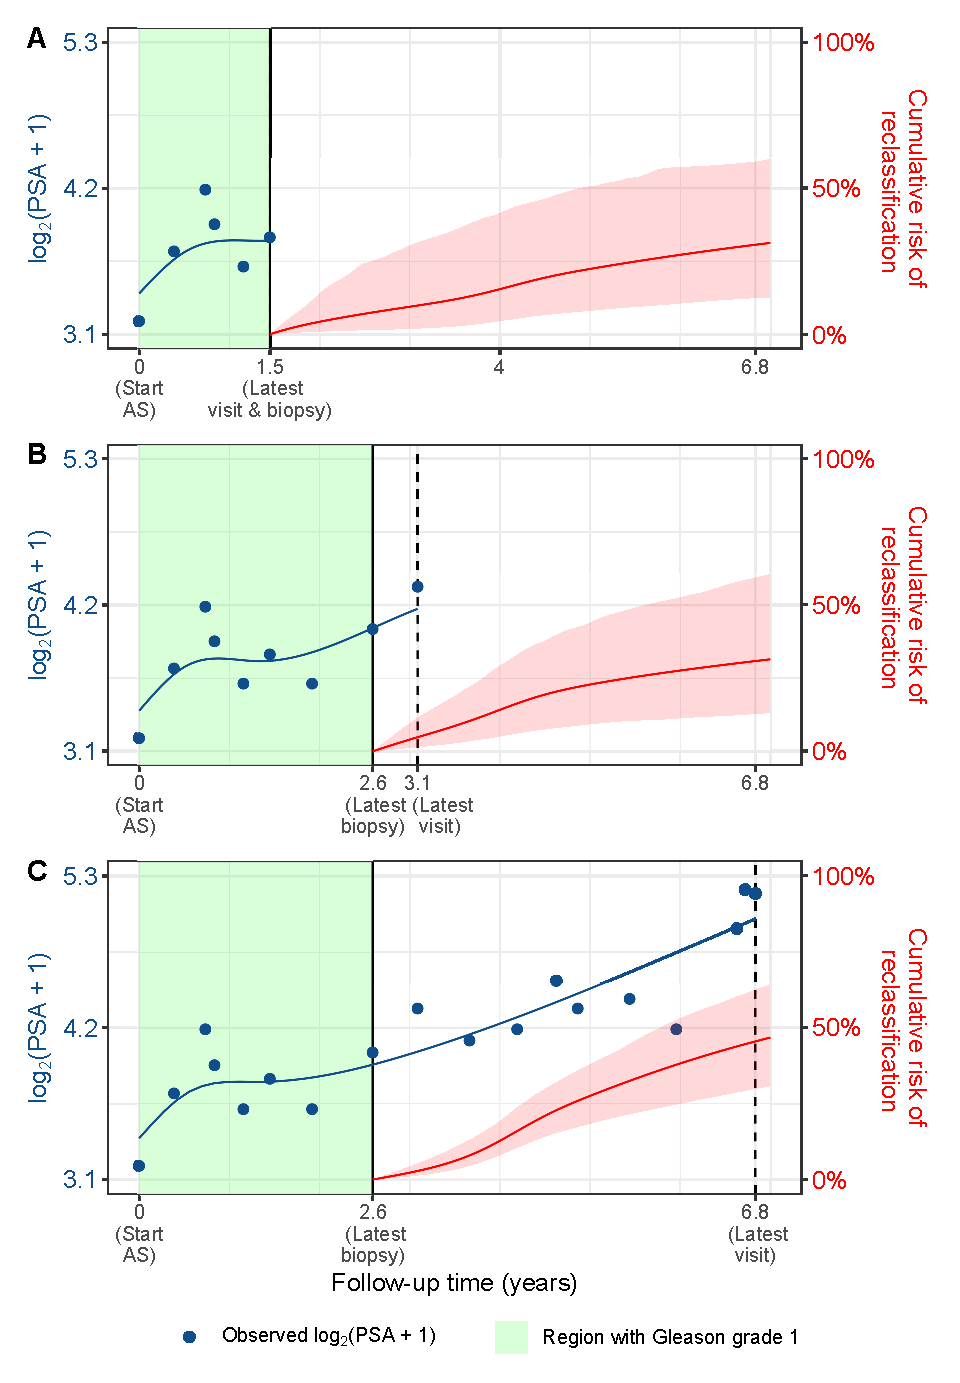
\includegraphics{images/dynrisk_plot_102.eps}}
\caption{\textbf{Cumulative-risk of progression changing dynamically over follow-up} as more patient data is gathered. A single longitudinal outcome, namely, a continuous biomarker of disease progression, is used for illustration. \textbf{Panels~A,~B~and~C:} are ordered by the time of the current visit (dashed vertical black line) of a new patient. At each of these visits, we combine the accumulated longitudinal measurements (shown in blue), and last time of negative invasive test (solid vertical green line) to obtain the updated cumulative-risk profile (shown in red) of the patient. All values are illustrative.} 
\label{fig:dynrisk_explanation}
\end{figure}

\subsection{Schedule of Invasive Tests}
\label{subsec:pers_schedule}
Our aim is to employ the cumulative-risk function in~(\ref{eq:cumulative_risk}) to develop a personalized schedule of invasive tests for the $j$-th patient. Typically invasive tests are planned on the same visit on which auxiliary data (e.g., biomarkers) is measured. Let $U={u_1, \ldots, u_L}$ represent a schedule of such visits (e.g., every six months in prostate cancer for PSA measurement), where $u_1=v$ is also the time of the current visit. In addition, $u_1 > t$, the time of the last test on which progression was not observed. We then propose scheduling future tests on all those visits in $U$ where the conditional cumulative-risk of progression is larger than a certain threshold $0 \leq \kappa \leq 1$ (e.g., $\kappa=10$\% risk). Each such future decision of a test at time $u_l \in U$ is given by:
\begin{equation*}
\label{eq:personalized_decision_grid}
\begin{split}
D_j(u_l \mid t_l, v, \kappa) &= I\big\{R_j(u_l \mid t_l, v) \geq \kappa \big\},\\
t_{l} &= \max \big\{t, u_m \mid D_j(u_m \mid t_m, v, \kappa)=1, m=1,\ldots,l-1 \big\}
\end{split}
\end{equation*}
where $D_j(u_l \mid t_l, v, \kappa)$ denotes the test decision at future visit time $u_l$, with 1 representing a test planned at $u_l$ and 0 otherwise, and $I(\cdot)$ is the corresponding indicator function. The conditional cumulative-risk of progression denoted by $R_j(u_l \mid t_l, v)$ is defined as in~(\ref{eq:cumulative_risk}). It is called `conditional' because test decision at each successive future visit time $u_l$ is made by accounting for the possibility that progression may not occur until the time of the last planned test $t_l$. That is, $T^*_j > t_l$. However, the contribution of the observed longitudinal data $\{\mathcal{Y}_{1j}(v), \ldots, \mathcal{Y}_{Kj}(v)\}$ does not change while making these consecutive decisions. The personalized schedule of tests $S_j^\kappa$ for a given risk threshold $\kappa$ is then defined as the subset of time points in $U$ on which tests are planned, until progression is observed or we reach a maximum horizon $h$.
\begin{equation*}
\label{eq:personalized_schedule_grid}
S_j^\kappa = \Big\{ u_l \in U \mid D_j(u_l \mid t_l, v, \kappa)=1, u_l < T^*_j, u_l<h \Big\}
\end{equation*}
Since the schedule is risk based, it also gets updated as more patient data becomes available over follow-up.

\begin{figure}
\centerline{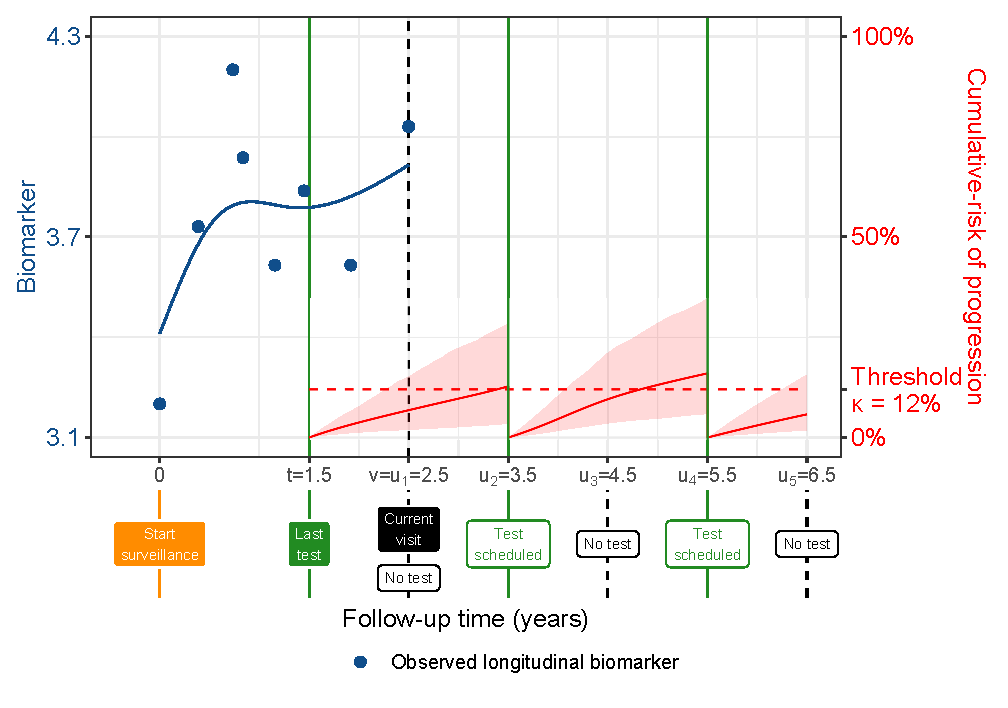
\includegraphics{images/schedule_explanation_102.eps}}
\caption{\textbf{Personalized Invasive Test Schedule Using Patient-specific Conditional Cumulative-risk of Progression}.  A single longitudinal outcome, namely, a continuous biomarker (observed: blue dots, fitted: blue line) of disease progression is used for illustration. The last test on which progression was not observed was conducted at $t=1.5$ years. The current visit time of the patient is $v=2.5$ years. Decisions for invasive test need to be made at a gap of every one year starting from the current visit until a horizon of 6.5 years. That is, $U=\{2.5, 3.5, 4.5, 5.5, 6.5\}$ years. Based on an example risk threshold of 12\% ($\kappa=0.12$) the future test decisions at time points in $U$ lead to a personalized schedule $S_j^\kappa = (3.8, 5.7)$ years. The conditional cumulative-risk profiles $R_j(u_l \mid t_l, v)$ employed in~(\ref{eq:personalized_decision_grid}) are shown with red line (confidence interval shaded). It is called `conditional' because, for example, the second test at future time 5.5 years, is scheduled after accounting for the possibility that progression (true time $T^*_j$) may not have occurred until the time of the previously scheduled test at time $3.5 < T^*_j$ years. All values are illustrative.} 
\label{fig:schedule_explanation}
\end{figure}

\subsection{Risk Threshold $\kappa$}
The risk threshold $\kappa$ controls the timing and the total number of invasive tests in the schedule $S_j^{\kappa}$. Through the timing of tests, $\kappa$ also indirectly affects the time delay (Figure~\ref{fig:delay_explanation}) that may occur in detecting progression if this schedule is followed. Hence, $\kappa$ should be chosen while balancing both the number of invasive tests (burden) and the time delay in detecting progression (less is beneficial).

Consider the bi-dimensional Euclidean space of the total number of invasive tests (x-axis) and the corresponding expected time delay in detecting progression (y-axis) for schedules associated with various $\kappa$ (Figure~\ref{fig:kappa_choice}). An ideal schedule of tests will have only one test planned exactly at the true time of progression $T^*_j$ of a patient. In other words, it will lead to a zero time delay. This schedule is shown at the point of optimality (1, 0) in Figure~\ref{fig:kappa_choice}. Subsequently, a threshold $\kappa_a$ can be chosen automatically by minimizing the Euclidean distance between the point $(1,~0)$ and the set of points representing various schedules corresponding to each $0 \leq \kappa \leq 1$. That is,
\begin{equation}
\label{eq:kappa_choice}
\kappa_a = \argmin_{\kappa} \sqrt{\big(\vert S_j^\kappa \vert - 1\big)^2 + \Big[E\{Q_j(S_j^{\kappa}, t)\} - 0\Big]^2} , \quad 0 \leq \kappa \leq 1,
\end{equation}
where, $E\{Q_j(S_j^{\kappa}, t)\}$ denotes the expected value of the time delay $Q_j(S_j^{\kappa}, t)$ in detecting progression if schedule $S_j^{\kappa}$ is followed. Additional consequences of following a particular schedule, such as (quality-adjusted) life-years saved, can also be accommodated in~(\ref{eq:kappa_choice}). This can be achieved by first setting a point of optimality in a higher dimensional Euclidean space of the aforementioned consequences, and then minimizing the Euclidean distance to the point of optimality.

Certain patients may have preferences for the maximum number of invasive tests scheduled for them. Others may be apprehensive about having an expected time delay higher than a certain number of months. In this regard, the Euclidean distance in~(\ref{eq:kappa_choice}) can be minimized under constraints on the number of tests and/or expected time delay (Figure~\ref{fig:kappa_choice}). An additional benefit of this approach is that it alleviates the issue of time delay and the number of tests having different units of measurement~\citep{cook1994equivalence}.

\begin{figure}
\centerline{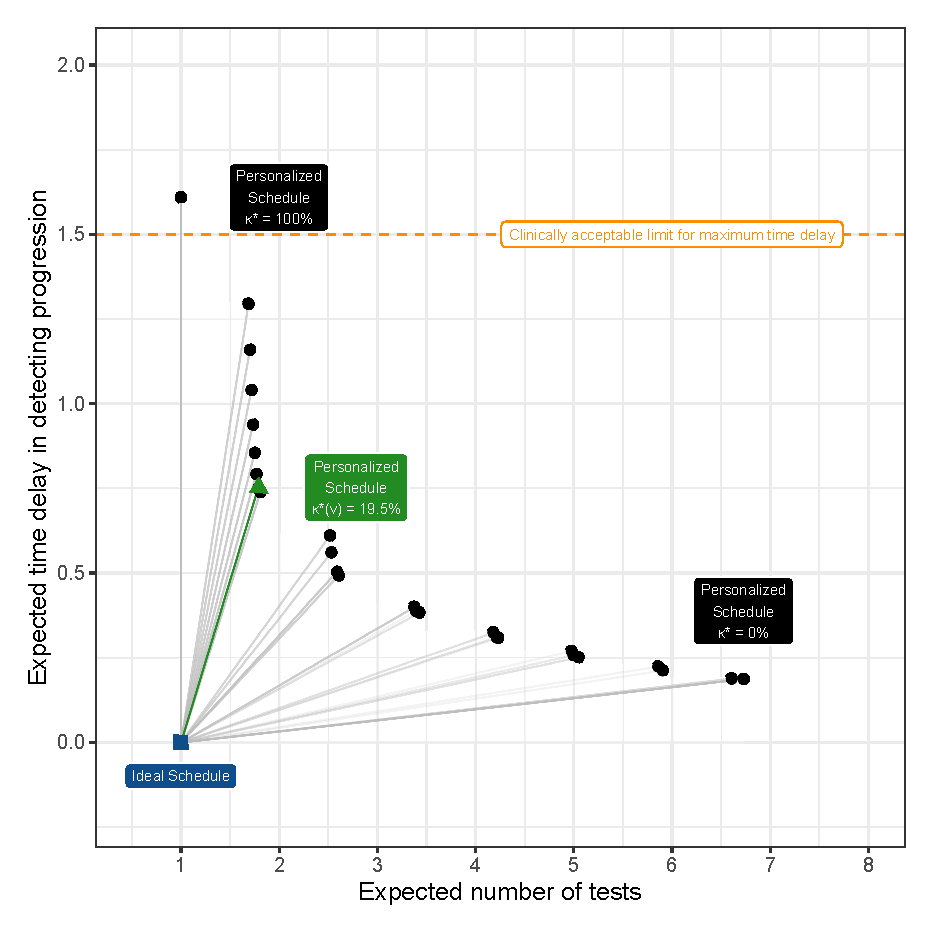
\includegraphics{images/kappa_choice_102.eps}}
\caption{\textbf{Automatic choice of risk threshold $0 \leq \kappa \leq 1$ using~(\ref{eq:kappa_choice})}. The ideal schedule of tests at point (1,0) is shown as a blue square. It plans exactly one invasive test at the true time of progression $T^*_j$ of a patient and hence leads to a zero time delay in detecting progression. Personalized schedules based on a grid of thresholds chosen between $0 \leq \kappa \leq 1$ are shown with black circles. Higher thresholds lead to fewer tests, but also higher expected time delay. We propose to choose the personalized schedule based on $\kappa_a=21.2\%$ threshold (green triangle). This is because it has the least Euclidean distance (shown with a green line) to the ideal schedule. It is also possible to find the least distance under a certain clinically acceptable limit on time delay (orange dashed line), or number of tests.}
\label{fig:kappa_choice}
\end{figure}

\subsection{Expected Time Delay in Detecting Progression}
\label{subsec:exp_delay_estimation}
Of the two measures in, we estimate the expected time delay in detecting progression $E\{Q_j(S_j^{\kappa}, t)\}$ in a patient-specific manner as well. That is, two patients may follow the same schedule, but they will expect different time delays. The calculation of the time delay is not limited to personalized schedules only, but can be done for any schedule $S$ with $N$ time points $S=\{s_1,\ldots, s_N\}$. Corresponding to each of these time points are the $N$ time intervals $s_{n-1} < T^*_j \leq s_n$ in which progression may be observed, and the $N$ possible time delays $s_n - T^*_j$, where $n=1,\ldots,N$. However, the time delay is not defined for the scenario in which the patient obtains progression after the time of the last test in the schedule $T^*_j > s_N$. The resulting definition for time delay given a schedule $S$ is:
\begin{equation}
Q_j (S, t) = \left\{ \begin{array}{lcrr}
  s_1 - T^*_j, &\mbox{if}& s_0 < T^*_j \leq s_1, &s_0=t\\
  \ldots \\
  s_N - T^*_j, &\mbox{if}& s_{N-1} < T^*_j \leq s_N  
\end{array} \right.
\end{equation}
We utilized the patient-specific expected time delay $E\{Q_j(S_j^{\kappa}, t)\}$ in~(\ref{eq:kappa_choice}). To this end, we exploit the personalized cumulative-risk profile of the patient (Equation~\ref{eq:cumulative_risk}). Specifically, the expected time delay can be calculated as the weighted sum of the $N$ conditional expected time delays, corresponding to the $N$ scenarios wherein the patient obtains progression in the intervals $s_{n-1} < T^*_j \leq s_n$, with $n=1,\ldots,N$.
\begin{equation}
\label{eq:expected_delay}
\begin{split}
E\{Q_j(S, t)\} &= \sum_{n=1}^{N} q_j(s_n, s_{n-1}) \mbox{Pr}(s_{n-1} < T^*_j \leq s_n) , \quad s_0 = t\\
q_j(s_n, s_{n-1}) &= s_n - E(T^*_j \mid s_{n-1}, s_n, v)\\
E(T^*_j \mid s_{n-1}, s_n, v) &= s_{n-1} + \int_{s_{n-1}}^{s_n} \mbox{Pr}\Big\{T^*_j \geq u \mid s_{n-1} < T^*_j \leq s_n, \mathcal{Y}_{1j}(v), \ldots, \mathcal{Y}_{Kj}(v), \mathcal{A}_n\Big\} \mathrm{d}u\\
\mbox{Pr}(s_{n-1} < T^*_j \leq s_n) &= R_j(s_n \mid t, v) - R_j(s_{n-1} \mid t, v),
\end{split}
\end{equation}
where $E(T^*_j \mid s_{n-1}, s_n, v)$ denotes the conditional expected time of progression for the scenario $s_{n-1} < T^*_j \leq s_n$, and is calculated as the area under the corresponding survival curve. The personalized expected delay has the advantage that it is updated over follow-up as more patient data becomes available. Since it can be calculated for any schedule, it can assist patients and doctors in comparing schedules before making a decision. Although, in order to have a fair comparison of expected delays between different schedules for the same patient, a compulsory test at a common horizon time point should be planned in all schedules.
% !TEX root =  ../main_manuscript.tex 
\section{Application of Personalized Schedules in Prostate Cancer Surveillance}
\label{sec:results}
We next demonstrate personalized schedules for scheduling biopsies in prostate cancer active surveillance. To this end, we reuse results from a joint model we previously fitted~\citep{tomer2019personalized} to the PRIAS dataset introduced in Section~\ref{sec:introduction}. This model utilized a linear mixed sub-model for biannually measured PSA (continuous: log-transformed from ng/mL), and a logistic mixed sub-model for biannually measured DRE (binary: tumor palpable or not). The model employed B-splines~\citep{de1978practical} to accommodate non-linear PSA evolution over follow-up. In the survival sub-model, fitted PSA value, fitted instantaneous PSA velocity (defined in Section~\ref{subsec:surival_sub_model}), and log-odds of having a DRE indicating a palpable tumor, were included as time-dependent predictors. The model parameters were estimated under the Bayesian framework~\citep{tomer2019personalized} using the R package \textbf{JMbayes}~\citep{rizopoulosJMbayes}. While the complete model definition and parameter estimates are provided in~\citet{tomer2019personalized}, we next briefly present the key results relevant for personalized scheduling.

First, the cause-specific cumulative-risk of cancer progression at the maximum study period of ten years was 50\% (Web-Figure~1). This indicates that many patients may not require all of the yearly biopsies they are usually prescribed. Since personalized schedules are risk-based, their overall performance is dependent on the predictive accuracy and discrimination capacity of the fitted model. In this regard, the model had a moderate area under the receiver operating characteristic curve (AUC) over the follow-up period (between 0.61 and 0.68). The mean absolute prediction error was moderate to large (between 0.08 and 0.24) and decreased rapidly after year one of the follow-up. Thus, personalized schedules based on this model may work better after year one with more follow-up data.

\subsection{Personalized Biopsy Schedules for a Demonstration Prostate Cancer Patient}
\label{subsec:demo_patient}
We utilized the joint model fitted to the PRIAS dataset to schedule biopsies in a demonstration prostate cancer patient shown in Figure~\ref{fig:demo_schedule}. The time of his last negative biopsy was $t=3.5$ years, and the time of the current visit was $v=5$ years. We made biopsy decisions over his future visits for PSA measurement $U=\{u_1=5, u_2=5.5,\ldots,u_L=10\}$ years using four different schedules. Two of the fixed schedules are annual biopsy schedule and the PRIAS schedule. The PRIAS schedule has compulsory biopsies at year one, four, seven, and ten of follow-up, and additional annual biopsies if PSA doubling-time~\citep{bokhorst2015compliance} is high. Remaining two schedules are personalized, namely, with a fixed threshold $\kappa=10\%$ risk, and an automatically chosen current visit time $v$ specific risk $\kappa^*(v)$ (Section~\ref{subsec:kappa_selection}). Since the demonstration patient's time of last negative biopsy $t=3.5$ is after year one of follow-up, a time delay in detecting progression
up to three years may not lead to adverse downstream outcomes~\citep{carvalho}.

\begin{figure}
\centerline{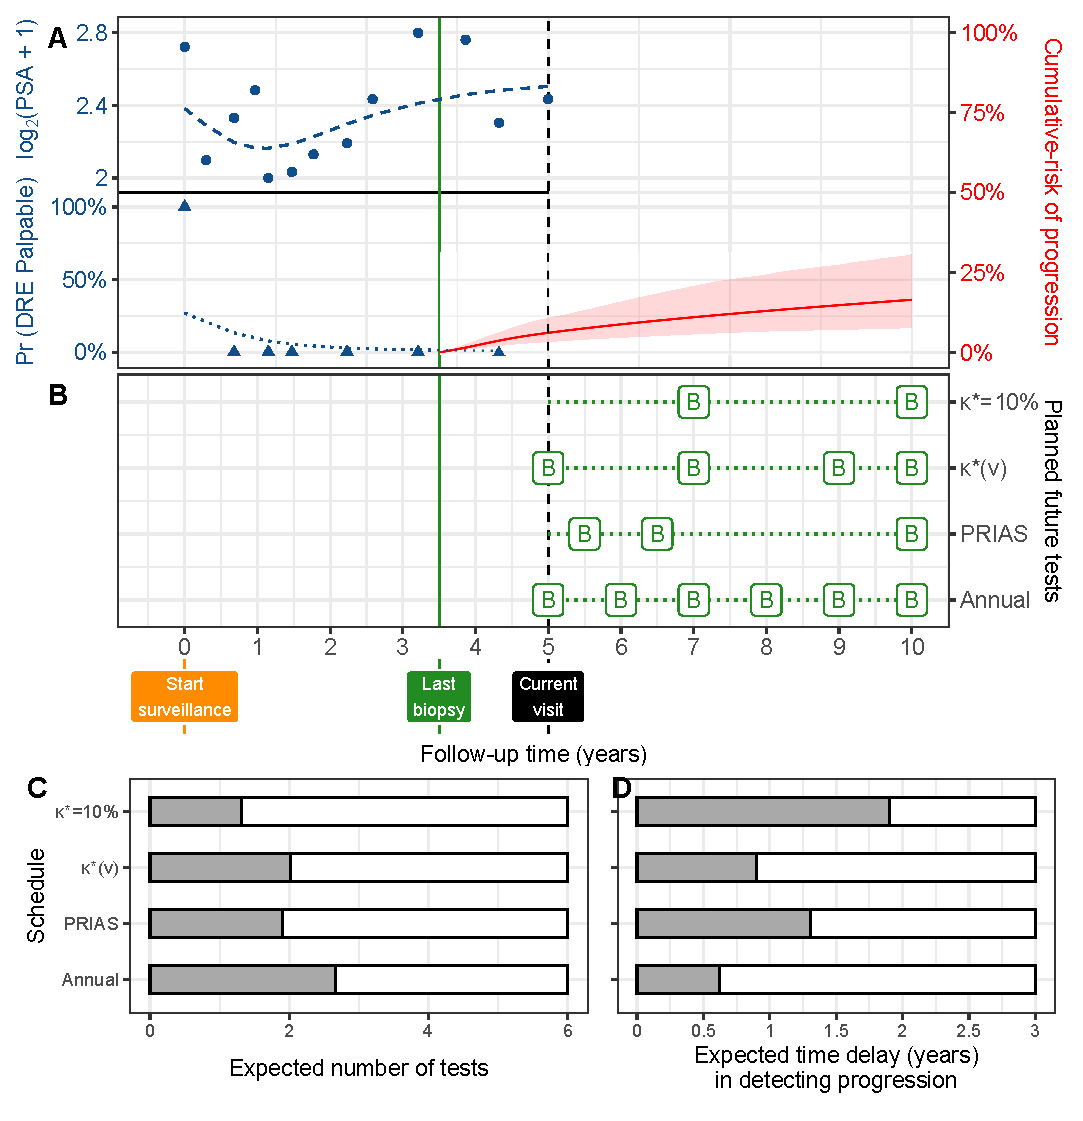
\includegraphics{images/demo_schedule.eps}}
\caption{\textbf{Personalized schedules for a demonstration prostate cancer patient}. \textbf{Panel~A}: Time of current visit: $v=5$ years (black dashed line). Time of last negative biopsy: $t=3.5$ years (vertical green solid line). Longitudinal data: $\log_2(\mbox{PSA} + 1)$ transformed~\citep{tomer2019personalized} PSA (observed: blue dots, fitted: dashed blue line), and binary DRE (observed: blue triangles, fitted probability: dotted blue line). Cumulative-risk profile: solid red line (95\% credible interval shaded). \textbf{Panel~B}: Different biopsy schedules are shown with a `B' indicating a biopsy. \textbf{$\kappa=10\%$} and \textbf{$\kappa^*(v)$} are personalized biopsy schedules using a risk threshold of 10\%, and a visit time $v$ specific automatically chosen threshold~(\ref{eq:kappa_choice}), respectively. PRIAS and Annual denote the PRIAS biopsy schedule (Section~\ref{subsec:demo_patient}) and annual biopsy schedule. \textbf{Panel~C,D}: For all schedules we calculate the expected number of tests and expected time delay in detecting progression if the patient progresses before year ten. Since a recommended minimum gap of one year is maintained between biopsies, maximum possible number of tests are six. A delay in detecting progression of up to three years may not lead to adverse outcomes~\citep{carvalho}. }
\label{fig:demo_schedule}
\end{figure}

The cumulative-risk of progression of the demonstration patient increases 3\% yearly on average, up to 19\% at the maximum study period of ten years. Hence, the patient may progress slowly. Consequently, risk-based personalized approaches plan fewer biopsies than the annual schedule (Panel~B, Figure~\ref{fig:demo_schedule}). Also, the time delay in detecting progression for personalized schedules (Panel~D, Figure~\ref{fig:demo_schedule}) is below the safe limit of three years mentioned earlier. Thus, personalized schedules can be a suitable alternative to the annual schedule.

\subsection{Web-application for Personalized Biopsy Schedules Prostate Cancer Surveillance}
We implemented the methodology for scheduling risk-based biopsies in prostate cancer active surveillance in a web-application (\url{https://emcbiostatistics.shinyapps.io/prias\_biopsy\_recommender/}). In this web-application, four types of risk-based personalized schedules are provided, namely, using 5\%, 10\%, and 15\% fixed thresholds, and a current-visit time specific optimal threshold obtained via~(\ref{eq:kappa_choice}). Also, a general purpose source code for creating personalized test schedules is provided in Web-Appendix~D. The source code is compatible with joint models fitted using the R package \textbf{JMbayes}~\citep{rizopoulosJMbayes}.
% !TEX root =  ../pers_schedules.tex 

\section{Simulation study}
\label{sec: simulation_study}
The application of personalized schedules for patients from PRIAS demonstrated that the schedules adapt according to the historical data of each patient. However we could not perform a full scale comparison between personalized and PRIAS schedules, because the true time of GR was not known for any of the PRIAS patients. To this end, we have performed a simulation study comparing personalized schedules based on expected time of GR, median time of GR and dynamic risk of GR with a mixed approach between median time of GR and dynamic risk of GR, PRIAS schedule and annual schedule. We employ these schedules for simulated patients enrolled in a hypothetical AS program, with the same entrance criteria as PRIAS.

\subsection{Simulation setup}
\label{subsec : simulation_setup}
\subsubsection{Patient population}
First we assume a population of patients enrolled in AS, whose PSA and hazard of GR follows a joint model of the form postulated in Section \ref{subsec : jm_fit_prias}, with parameters equal to the posterior mean of parameters (CHECK WEB SUPPLEMENTARY SECTION...) estimated from the joint model fitted to PRIAS dataset. We assume that the patients in population belong to 3 equal sized subgroups $G_1, G_2, G_3$ with different failure times. The failure times are controlled by different Weibull distributed baseline hazards for each. The shape and scale parameters $(k, \lambda$) for the 3 subgroups are: $(1.5, 4)$, $(3, 5)$ and $(4.5, 6)$ for $G_1, G_2$ and $G_3$ respectively. The effect of these parameters is that the variance in GR times is highest for $G_1$ and lowest for $G_3$, while the mean GR time is lowest in $G_1$ and highest in $G_3$.

From the population we randomly sample a total of 408 datasets with 1000 patients each. Each dataset is split into a training (750 patients) and a test (250 patients) part. The $k$-th simulated training dataset $\mathcal{D}^k$ is given by $\mathcal{D}^k = \{l_{ki}, r_{ki}, \boldsymbol{y}_{ki}; i = 1, \ldots, 750\}$, where $\boldsymbol{y}_{ki}$ denote the PSA measurements for the $i$-th patient in $\mathcal{D}^k$. The frequency of PSA measurements is same as that in PRIAS. Other than simulating a true GR time $T^*_{ki}$, we also generate a random and non-informative censoring time $C_{ki}$. When $T_{ki} < C^*_{ki}$, then $l_{ki} = r_{ki} = T^*_{ki}$, otherwise $l_{ki} = C_{ki}$ and $r_{ki} = \infty$. For the test patients, censoring time is not generated.

Next we fit a joint model of the specification given in \ref{eq : long_model_prias} and \ref{eq : hazard_prias} to each of the $\mathcal{D}^k, k=1,
\ldots, 408$, and obtain posterior distribution of parameters $p(\boldsymbol{\theta} \mid \mathcal{D}^k)$. Using the latter, we obtain the PPD $g(T^*_{kj})$ for the $j$-th test patient and conduct hypothetical biopsies iteratively in accordance with the algorithm in Figure \ref{fig : sched_algorithm}. 

\subsection{Estimation}
For estimation of the optimal $\kappa = \argmax_{\kappa} F_1(t, \Delta t, s)$, we use a grid search approach. That is, $F_1$ is computed using the training dataset over a fine grid of $\kappa$ values in the interval $[0,1]$  and then the most optimal value is chosen.

The next step is to estimate the measures of efficacy of schedules. To this end, we estimate $E[N^{bS}]$, $\mbox{var}[N^{bS}]$, $E[O^S]$ and $\mbox{var}[O^S]$ using pooled estimates of each from the 408 test datasets, as follows:
\begin{align*}
\widehat{E[O^S]} &= \frac{\sum_{k=1}^{254} n_k \widehat{E[O^S_k]}}{\sum_{k=1}^{254} n_k}, \\
\widehat{\mbox{var}[O^S]} &= \frac{\sum_{k=1}^{254} (n_k - 1) \widehat{\mbox{var}[O^S_k]}}{\sum_{k=1}^{254} (n_k-1)}, 
\end{align*}
where $n_k$ are the number of test patients in the $k$-th simulation, $\widehat{E[O^S_k]} = {\sum_{j=1}^{n_k}O^S_{kj}}/{n_k}$ is the estimated mean and $\widehat{\mbox{var}[O^S_k]} = {\sum_{j=1}^{n_k}\big\{O^S_{kj} - \widehat{E[O^S_k]}\big\}^2}/{n_k-1}$ is estimated variance of the offset for the $k$-th simulation. The estimates for number of biopsies $N^{bS}$ are obtained similarly.

\subsection{Results}
From the simulations we calculated the pooled estimates of the mean and variance of number of biopsies/offset for the entire sample. The estimates are plotted in Figure \ref{fig : meanNbVsOffset} and also summarized in Table \ref{table : sim_study_pooled_estimates}. From the figure it is evident that those schedules which conduct less biopsies on average, have a higher average offset, and vice versa. For example, the annual schedule conducts 5.2 biopsies on average, which is the highest among all schedules, however it has the least average offset of 6 months as well. On the other hand the schedule based on expected time of GR conducts only 1.9 biopsies on average, the least among all schedules but it also has the highest average offset of 15 months. The schedule based on median time of GR performs almost the same as that based on expected time of GR. As mentioned earlier the variance in number of biopsies and offset are important as well. In this regard annual schedule has the largest $\mbox{var}[N^{bS}]$ since it attempts to contain the offset within an year, and consequently it has the least $\mbox{var}[O^S]$. Schedules based on expected and median time of GR perform the opposite in terms of variance.

\begin{figure}
	\centerline{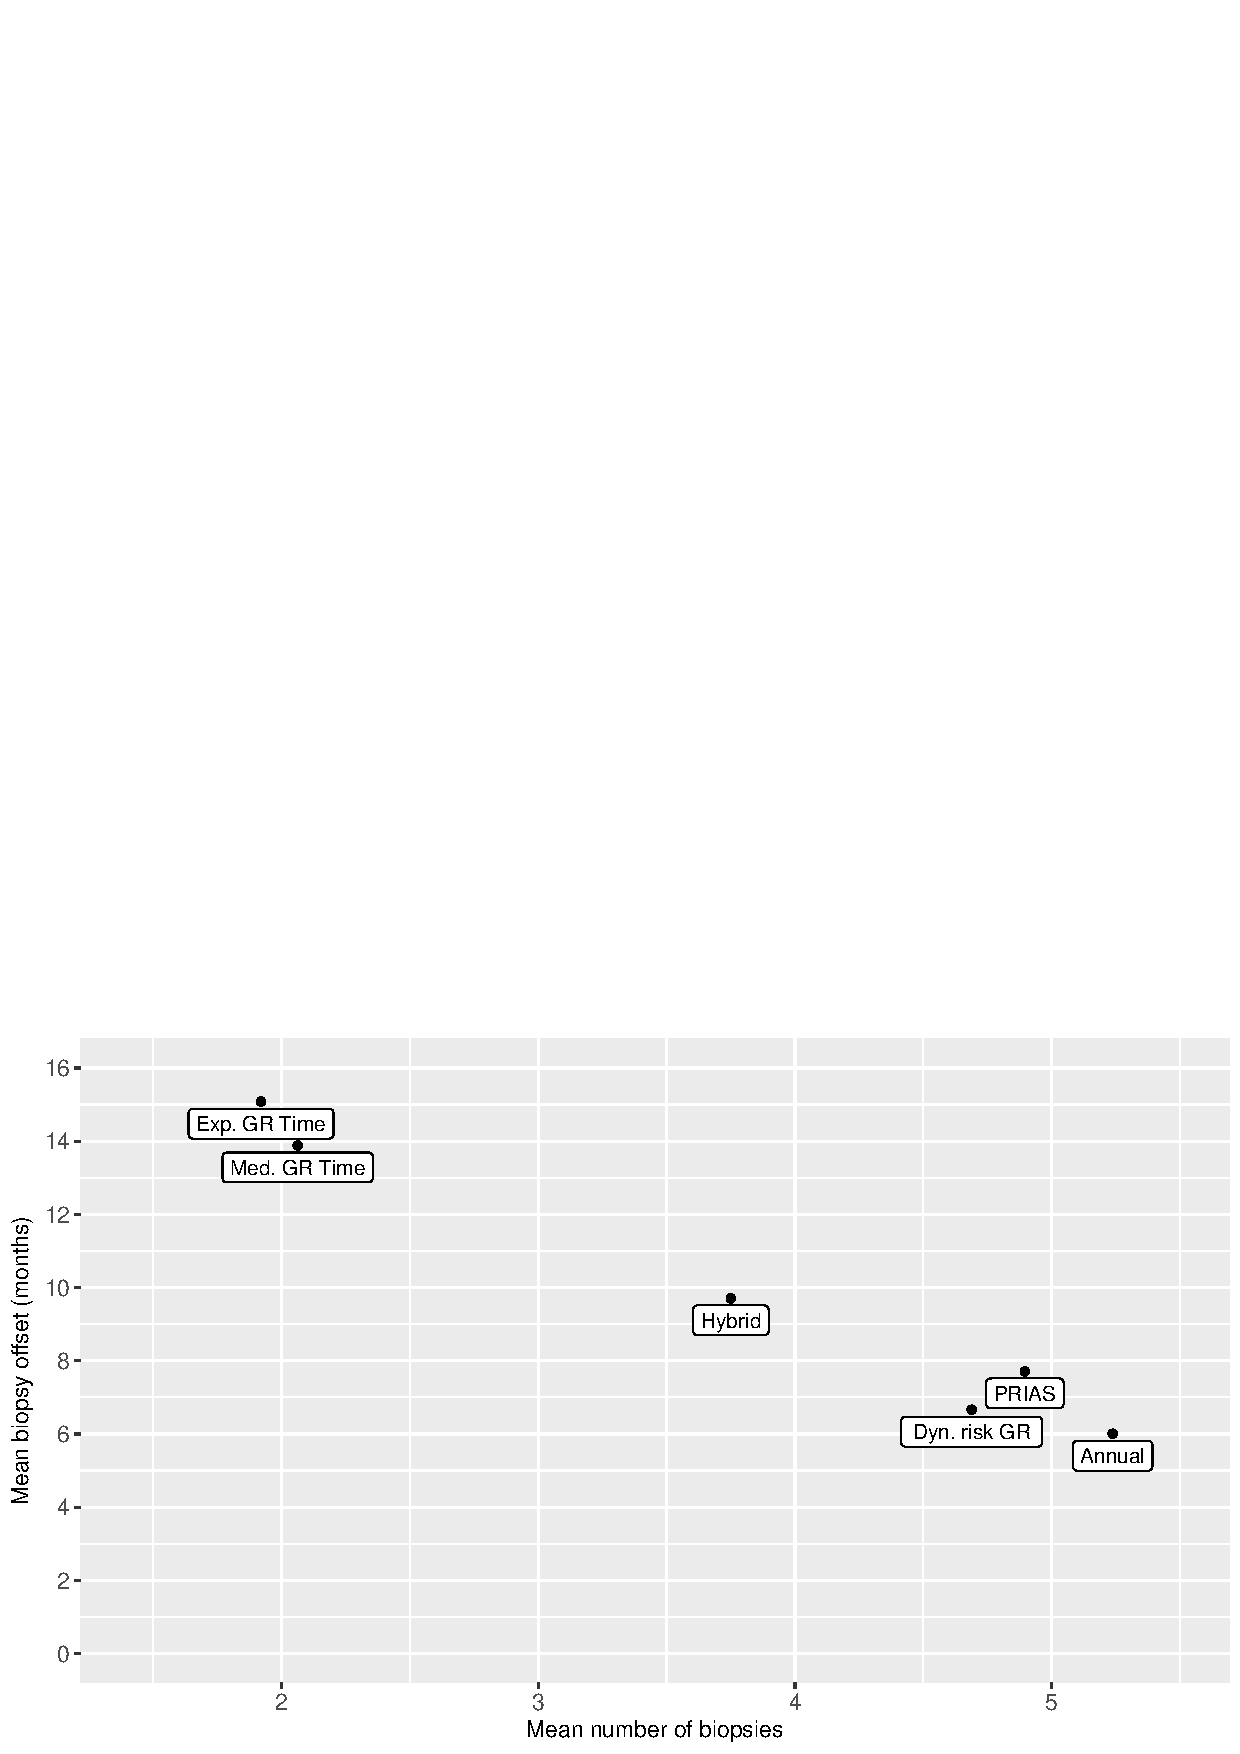
\includegraphics[width=\columnwidth]{images/sim_study/meanNbVsOffset_all.png}}
	\caption{Estimated mean number of biopsies and mean offset (months) for the 7 scheduling methods using all patients. Method names are abbreviated for ease of graphing.}
	\label{fig : meanNbVsOffset}
\end{figure}

\begin{table}
\caption{Pooled estimates of mean and variance of number of biopsies and offset for all patients.}
\label{table : sim_study_pooled_estimates}
\begin{tabular}{lrrrr}
\Hline
Schedule          & $E[N^{bS}]$ & $E[O^{S}]$ & $\mbox{var}[N^{bS}]$ & $\mbox{var}[O^S]$ \\  \hline
Annual & 5.23           & 6.00               & 6.42          & 11.87             \\
PRIAS & 4.85           & 8.46               & 5.52          & 74.22             \\
Expected time of GR & 1.92           & 15.06              & 1.42          & 146.31          \\
Median time of GR  & 2.06           & 13.89              & 2.00          & 139.73            \\
$\text{F}_1$-Score  & 4.68           & 6.65               & 4.80          & 18.83             \\
Mixed approach & 3.76          & 9.74               & 2.88          & 58.35             \\
\hline
\end{tabular}
\end{table}

We observe that the PRIAS schedule performs more or less the same as annual schedule. Despite this the latter may be preferred over PRIAS since it conducts only 0.38 biopsies more on average, however unlike PRIAS it has very low variance of offset, thus guaranteeing early detection for everyone. If we compare the PRIAS schedule with dynamic risk of GR based schedules, we can see that the schedule where $\kappa$ is chosen after maximizing $\text{F}_1$-Score, performs better than in PRIAS schedule in all aspects. The schedule where $\kappa$ is chosen after maximizing Youden's $J$ has a very large $\mbox{var}[O^S]$ and hence is not preferable over PRIAS. The mixed approach combines the benefits of methods with low $E[N^{bS}]$ and $\mbox{var}[N^{bS}]$, and those methods with low $E[O^{S}]$ and $\mbox{var}[O^S]$. It conducts 1.5 less biopsies than annual schedule on average and at 9.7 months the mean offset is less than an year.

\begin{table}
\caption{Pooled estimates of mean and variance of number of biopsies and offset for subgroup $G_1$.}
\label{table : sim_study_pooled_estimates_G1}
\begin{tabular}{lrrrrr}
\Hline
Schedule           & Total Patients & $E[N^{bS}]$ & $E[O^{S}]$ & $\mbox{var}[N^{bS}]$ & $\mbox{var}[O^S]$ \\  \hline
Annual              & 21004                  & 4.306           & 6.024               & 9.788          & 11.747             \\
PRIAS              & 21004                  & 4.032           & 7.951               & 8.221          & 63.528             \\
Expected time of GR & 21001                  & 1.922           & 15.114              & 1.441          & 149.167            \\
Median time of GR  & 20937                  & 2.068           & 13.87               & 1.999          & 138.396            \\
$\text{F}_1$-Score           & 21061                  & 4.689           & 6.648               & 4.863          & 18.745             \\
Mixed approach     & 21004                  & 3.252           & 10.361              & 4.611          & 73.781             \\
\hline
\end{tabular}
\end{table}

\begin{table}
\caption{Pooled estimates of mean and variance of number of biopsies and offset for subgroup $G_2$.}
\label{table : sim_study_pooled_estimates_G2}
\begin{tabular}{lrrrrr}
\Hline
Schedule           & Total Patients & $E[N^{bS}]$ & $E[O^{S}]$ & $\mbox{var}[N^{bS}]$ & $\mbox{var}[O^S]$ \\  \hline
Annual              & 21160                  & 5.181           & 5.95                & 4.567          & 12.03              \\
PRIAS              & 21160                  & 4.817           & 8.569               & 3.98           & 75.716             \\
Expected time of GR & 21151                  & 1.927           & 15.078              & 1.447          & 144.333            \\
Median time of GR  & 21189                  & 2.062           & 13.947              & 1.994          & 140.633            \\
$\text{F}_1$-Score           & 21133                  & 4.666           & 6.663               & 4.726          & 18.956             \\
Mixed approach     & 21160                  & 3.702           & 10.359              & 1.869          & 60.415             \\
\hline
\end{tabular}
\end{table}

\begin{table}
\caption{Pooled estimates of mean and variance of number of biopsies and offset for subgroup $G_3$.}
\label{table : sim_study_pooled_estimates_G3}
\begin{tabular}{lrrrrr}
\Hline
Schedule           & Total Patients & $E[N^{bS}]$ & $E[O^{S}]$ & $\mbox{var}[N^{bS}]$ & $\mbox{var}[O^S]$ \\  \hline
Annual              & 21222                  & 6.214           & 6.03                & 3.118          & 11.851             \\
PRIAS              & 21222                  & 5.717           & 8.866               & 2.977          & 82.915             \\
Expected time of GR  & 21234                  & 1.921           & 15.006              & 1.375          & 145.426            \\
Median time of GR   & 21260                  & 2.07            & 13.879              & 2.016          & 140.14             \\
Youden's $J$              & 21202                  & 4.541           & 8.02                & 4.061          & 112.559             \\
Mixed approach     & 21222                  & 4.33            & 8.521               & 1.581          & 38.586             \\
\hline
\end{tabular}
\end{table}

We next check the performance of these methods for each of the 3 subgroups $G_1, G_2$ and $G_3$. Estimates of $E[N^{bS}]$, $\mbox{var}[N^{bS}]$, $E[O^S]$ and $\mbox{var}[O^S]$ for the 3 subgroups are presented in Table \ref{table : sim_study_pooled_estimates_G1}, Table \ref{table : sim_study_pooled_estimates_G2} and Table \ref{table : sim_study_pooled_estimates_G3}. We observe that all of the schedules which are based on personalized methods, i.e. expected time of GR, median time of GR and dynamic risk of GR based schedules perform the same across the subgroups, with trivial differences in estimates. On the other hand, the annual schedule conducts 6 biopsies on average for patients in $G_3$ as compared to 4 for patients in $G_1$. It also has $\mbox{var}[N^{bS}]$ 3 times more for patients in $G_1$ compared to $G_3$. This can be attributed to the former having higher variance in GR times. However for annual schedule the $E[O^S]$ and $\mbox{var}[O^S]$ remain almost the same in all groups and it always detects GR within an year of the occurrence. The PRIAS schedule differs for the 3 subgroups as well. For number of biopsies the dynamics are similar to that of annual schedule. However for offset, the PRIAS schedule has high $E[O^S]$ and $\mbox{var}[O^S]$ for patients from $G_3$, i.e. patients who obtain GR later. As for the mixed approach, we observe that it conducts more biopsies on average for patients from $G_3$, however it also has the least $E[O^S]$, $\mbox{var}[O^S]$ and $\mbox{var}[N^{bS}]$ for the same group.

To assess the methods further, we combined data from all of the 63386 patients, and also plotted the box plots for number of biopsies and offset in Figure \ref{fig : nbBoxPlot} and Figure \ref{fig : offsetBoxPlot} respectively. Based on the combined data, we observe that both expected and median failure time of GR based schedules have 91.7\% and 92.5\% of patients below offset cutoff of 36 months, respectively. They also have 80.5\% and 82.3\% of patients below a cutoff of 24 months. Thus they seem to be quite practical. The mixed approach offers another practically viable solution, since neither it has large $\mbox{var}[N^{bS}]$, nor $\mbox{var}[O^S]$. The estimated $E[N^{bS}]$ is 3.8 and the estimated $E[O^S]$ is 9.7 months. For 99.9\% patients it has an offset below 36 months and for 95\% patients it has an offset below 24 months. Given this offset and the fact that it conducts much less biopsies than PRIAS schedule, annual schedule, and dynamic risk of GR based schedules, it is preferable over them.
% !TEX root =  ../main_manuscript.tex 
\section{Discussion}
We developed a novel methodology for personalized biopsies in low-risk PCa patients enrolled in AS programs. These biopsies are based on a patient's risk profile for having a Gleason $\geq$ 7 (GS7). To assist patients in making a choice between the personalized and currently practiced fixed schedules, we give objective estimates of the consequences of following each schedule. More specifically, for a schedule we give the total number of biopsies (burden), the time at which they will be conducted, and the expected delay in detection of GS7. This delay is estimated after accounting for the probability of not having any GS7 at all over the follow-up period. Lastly, our approach dynamically updates the aforementioned schedules and consequences as more patient data becomes available over follow-up.

The aforementioned methodology is based on the world's largest PCa AS program, PRIAS. Consequently, a lot of patients may get benefited from this study. To this end, we have developed a web-application implementing our methodology. The web-application only requires patient data in well known file formats (e.g., SPSS, CSV etc.), but does not require any separate integration with the electronic health record of the PRIAS program. We hope that this will lead to improvement in the shared decision making of biopsies, with patients having objective estimates of the consequences of their decisions. 

\textbf{Clinical implications:} The median survival time for GS7 is more than ten years in PRIAS. That is, more than 50\% patients do not require any biopsy during the first ten years of follow-up. The situation is similar in many other cohorts. Hence frequent biopsies may not be recommended for all patients.

Existing work on reducing the burden of biopsies in AS primarily advocates less frequent heuristic schedules of biopsies \citep{inoue2018comparative} (e.g., biopsies biennially instead of annually). To our knowledge, risk-based biopsy schedules have barely been explored yet in AS \citep{nieboer2018active,bruinsma2016active}. The part of our results pertaining to the fixed/heuristic schedules is comparable with corresponding results obtained in existing work \citep{inoue2018comparative}, even though the AS cohorts are not the same. Thus, we anticipate similar validity for the results pertaining to the personalized schedules.

Our work has certain limitations. The prediction model that we developed is valid only for the first thirteen years of follow-up in AS, whereas PCa in AS patients progresses slowly. This issue can be mitigated by refitting the model as more follow-up data is gathered in PRIAS. The results of external validation indicate that the use of our model may be restricted in cohorts with AUC, and RMSPE results similar to that of PRIAS. To this end, in other cohorts, refitting the model to their dataset will be required before making risk based schedules, and estimating the consequences of each schedule. There is also a potential for including diagnostic information from novel biomarkers, quality of life measures, and magnetic resonance imaging. Currently, this data is very sparsely available in the PRIAS dataset. However, in future, adding this information in our model is trivial. This is because modeling correlation for extra outcomes  (see Figure \ref{fig:jm_blockdiag}), mainly entails sharing the random effects in the joint model structure. Since MRI scans are expensive in developing countries, our model can also be used to trigger MRI scans. Lastly, in this study focus only on biopsy Gleason upgrade (reclassification). In this regard, accounting for competing risks (see Table \ref{table:prias_summary}), and for inter-observer variation \citep{coley2017prediction} in biopsy Gleason scores can be interesting to investigate further.

\section*{Acknowledgments}
The first and last authors would like to acknowledge support by Nederlandse Organisatie voor Wetenschappelijk Onderzoek (the national research council of the Netherlands) VIDI grant nr. 016.146.301, and Erasmus University Medical Center funding. Part of this work was carried out on the Dutch national e-infrastructure with the support of SURF Cooperative. The authors also thank the Erasmus University Medical Center's Cancer Computational Biology Center for giving access to their IT-infrastructure and software that was used for the computations and data analysis in this study.

This work was supported by the Movember Foundation. The funder did not play any role in the study design, collection, analysis or interpretation of data, or in the drafting of this paper.
\section*{Data Availability}
This work utilized results from a statistical model we previously fitted to the PRIAS dataset~\citep{tomer2019personalized}. The PRIAS database is not openly accessible. However, access to the database can be requested on the basis of a study proposal approved by the PRIAS steering committee. The website of the PRIAS program is \url{www.prias-project.org}. For sake of completeness and reproducibility of results, we have presented the PRIAS based model's definition and parameter estimates in Web-Appendix~B. The data of the demonstration patient in Figure~\ref{fig:demo_schedule} is provided in Web-Appendix~B.

\section*{Supporting Information}
Web Appendices referenced in this paper are available in the file titled `supplementary.pdf'.

\bibliographystyle{Chicago}

\bibliography{bibliography}
\end{document}
